\documentclass{article}

% Formatting
\usepackage[utf8]{inputenc}
\usepackage[margin=1in]{geometry}
\usepackage[titletoc,title]{appendix}

% Math
\usepackage{amsmath,amsfonts,amssymb,mathtools}

% Algorithms
\usepackage[ruled,vlined]{algorithm2e}
\usepackage{algorithmic}
\usepackage{listings}

% Code syntax highlighting
\usepackage{minted}
\usemintedstyle{borland}

% Tree & Forest
\usepackage[edges]{forest}

\title{Homework 5}
\author{David Trinh}
\date{October 21, 2024}

\begin{document}

\maketitle

\begin{itemize}

    \item\textbf{ Question 1}

        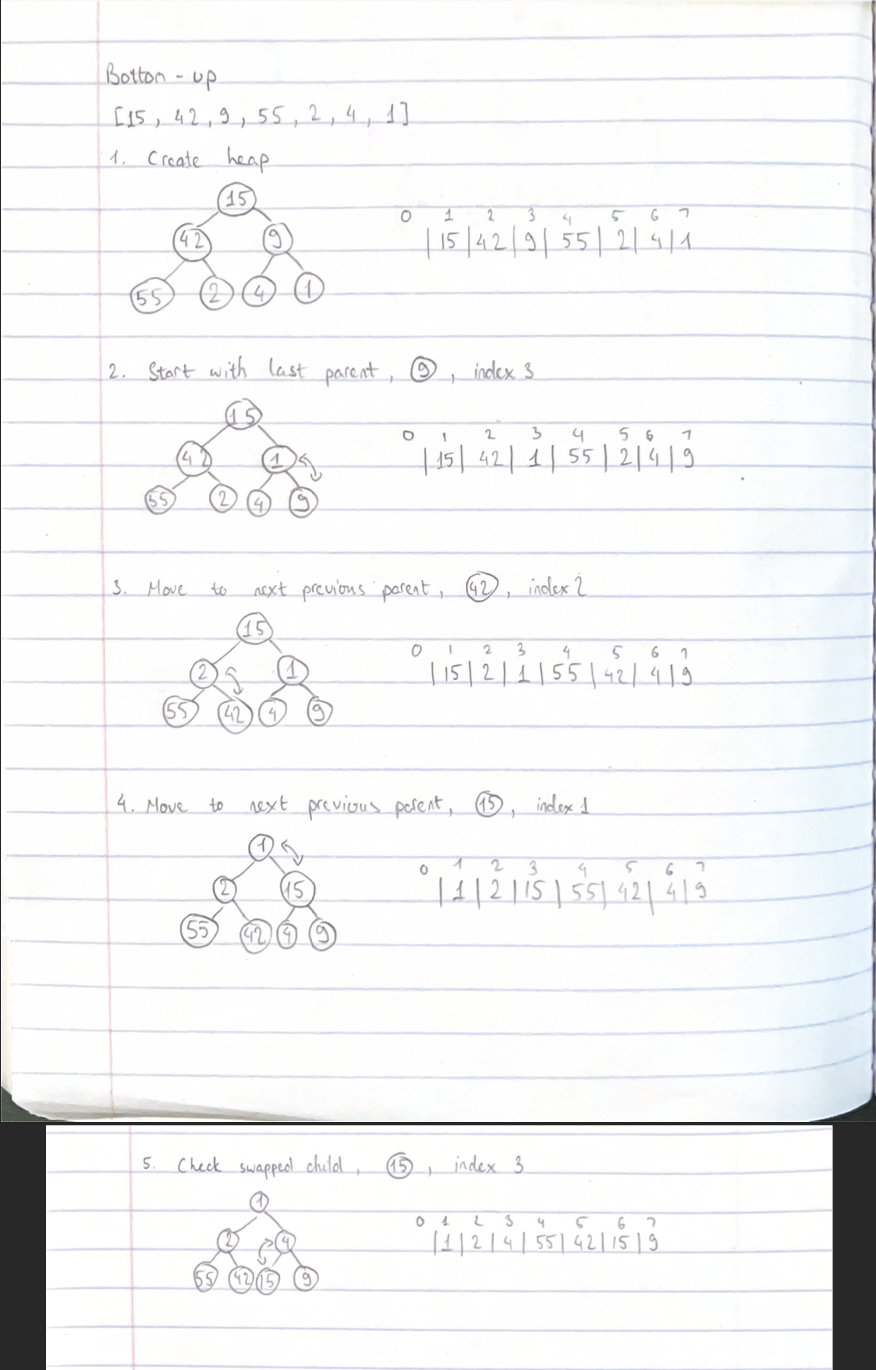
\includegraphics[scale=0.72]{HW5_Q1.png}

    \item\textbf{ Question 2}

    \begin{enumerate}
        \item { [1, 2, 3, 55, 42, 15, 9] }
        \item { [9, 2, 3, 55, 42, 15] 1 }
        \item { [2, 9, 3, 55, 42, 15] 1 }
        \item { [15, 9, 3, 55, 42] 1, 2 }
        \item { [3, 9, 15, 55, 42] 1, 2 }
        \item { [42, 9, 15, 55] 1, 2, 3 }
        \item { [9, 42, 15, 55] 1, 2, 3 }
        \item { [55, 42, 15] 1, 2, 3, 9 }
        \item { [15, 42, 55] 1, 2, 3, 9 }
        \item { [55, 42] 1, 2, 3, 9, 15 }
        \item { [42, 55] 1, 2, 3, 9, 15 }
        \item { [55] 1, 2, 3, 9, 15, 42 }
        \item { 1, 2, 3, 9, 15, 42, 55 }
    \end{enumerate}
    


    \item\textbf{ Question 3}


    \begin{enumerate}

        \item[] Backward
        \item[] $T(n) = 2T(\frac{n}{2}) + 5$, $T(1) = 0$
        \item[] $T(n/2) = 2T(\frac{n}{4}) + 5$
        \item[] $T(n/4) = 2T(\frac{n}{8}) + 5$
        \item[] $T(n/8) = 2T(\frac{n}{16}) + 5$
        \item[] $T(n/16) = 2T(\frac{n}{32}) + 5$
        \item[] ...
        \item[] Substitute
        \item[] $T(n) = 2T(\frac{n}{2}) + 5$
        \item[] $= 2(2T(\frac{n}{4}) + 5) + 5 = 4T(\frac{n}{4}) + 15$
        \item[] $= 4(2T(\frac{n}{8}) + 5) + 15 = 8T(\frac{n}{8}) + 35$
        \item[] $= 8(2T(\frac{n}{16}) + 5) + 35 = 16T(\frac{n}{16}) + 75$
        \item[] $= 16(2T(\frac{n}{32}) + 5) + 75 = 32T(\frac{n}{32}) + 155$
        \item[] ...
        \item[] Pattern
        \item[] $2^i T(\frac{n}{2^i}) + ( 2^i - 1 )5$
        \item[] $T(1) = T(\frac{n}{2^i}) \rightarrow 1 = n/2^i, n = 2^i, i = \log_2n$
        \item[] Plug in and solve
        \item[] $2^{ \log_2n } T(\frac{n}{2^{ \log_2n }}) + ( 2^{ \log_2n } - 1 )5$
        \item[] $n T(\frac{n}{n}) + ( n - 1 )5$
        \item[] $0 + ( n - 1 )5$
        \item[] $5n - 5$
        \item[] $\Theta (n)$
        \item[]
        \item[] Forward
        \item[] $T(1) = 0$
        \item[] $T(2) = 2T(1) + 5 = 5$
        \item[] $T(4) = 2T(2) + 5 = 15$
        \item[] $T(8) = 2T(4) + 5 = 35$
        \item[] $T(16) = 2T(8) + 5 = 75$
        \item[] $T(32) = 2T(16) + 5 = 155$
        \item[] Pattern
        \item[] $T(n) = 5n - 5$
        \item[] $\Theta (n)$
        \item[]
        \item[] In both the Backward and Forward steps
        \item[]
        \item[] Master Theorem
        \item[] $T(n) = 2T(\frac{n}{2}) + 5$
        \item[] $a = 2, b = 2, d = 0$
        \item[] $2 > 2^0$
        \item[] $\Theta (n^{\log_22})$
        \item[] $\Theta (n)$
        \item[] Therefore all the steps above are correct.

    \end{enumerate}

    \item\textbf{ Question 4}

    \begin{enumerate}
        \item $9T(\frac{n}{3}) + 27n^3$

            $a = 9, b = 3, d = 3$

            $9 < 3^3$

            $\Theta (n^3)$

        \item $0.5T(\frac{n}{0.9}) + n^n$

            $a = 0.5, b = 0.9, d = n$

            $a < 1, b < 1$

            MT

        \item $-2T(\frac{n}{2}) + \log_4n$

            $a = -2, b = 2$

            $a < 1, f(n)$ not in $\Theta ( n^d )$

            MT

        \item $4T(\frac{n}{2}) + n^2$

            $a = 4, b = 2, d = 2$

            $4 = 2^2$

            $\Theta (n^2logn)$

    \end{enumerate}

    \item\textbf{ Question 5}

    \begin{enumerate}
        \item Index: {\space 0, \space i, \space2, \space3, \space4, \space\space5, \space\space6, \space7, \space8, \space\space j}
    
            Value: {31, 37, 12, 3, 44, 50, 22, 39, 10, 25}

        \item Index: {\space 0, \space i, \space2, \space3, \space4, \space\space5, \space\space6, \space7, \space8, \space\space j}
    
            Value: {31, 25, 12, 3, 44, 50, 22, 39, 10, 37}

        \item Index: {\space 0, \space1, \space2, \space3, \space i, \space\space5, \space\space6, \space7, \space j, \space\space9}
    
            Value: {31, 25, 12, 3, 10, 50, 22, 39, 44, 37}

        \item Index: {\space 0, \space1, \space2, \space3, \space4, \space\space i, \space\space j, \space7, \space8, \space\space9}
    
            Value: {31, 25, 12, 3, 10, 22, 55, 39, 44, 37}

        \item Index: {\space 0, \space1, \space2, \space3, \space4, \space\space j, \space\space i, \space7, \space8, \space\space9}
    
            Value: {31, 25, 12, 3, 10, 55, 22, 39, 44, 37}

        \item Index: {\space 0, \space1, \space2, \space3, \space4, \space\space j, \space\space i, \space7, \space8, \space\space9}
    
            Value: {31, 25, 12, 3, 10, 22, 55, 39, 44, 37}

        \item Index: {\space j, \space1, \space2, \space3, \space4, \space left, \space\space i, \space7, \space8, \space\space9}
    
            Value: {22, 25, 12, 3, 10, 31, 55, 39, 44, 37}

    \end{enumerate}

    \item\textbf{ Question 6}

    \begin{enumerate}
        \item Low = 0, Mid = 4, High = 9, i = 0, j = 0, k = 0
        
            Index: {\space 0, \space 1, \space2, \space3, \space4, \space\space5, \space\space6, \space7, \space8, \space\space 9}
    
            Value: {3, 18, 25, 44, 51, 10, 12, 21, 36, 39}

        \item i = 0, j = 0, k = 0
        
            Index: {\space 0, \space 1, \space2, \space3, \space4, \space\space5, \space\space6, \space7, \space8, \space\space 9}
    
            Value: {3, 18, 25, 44, 51, 10, 12, 21, 36, 39}

        \item i = 1, j = 0, k = 1
        
            Index: {\space 0, \space 1, \space2, \space3, \space4, \space\space5, \space\space6, \space7, \space8, \space\space 9}
    
            Value: {3, 18, 25, 44, 51, 10, 12, 21, 36, 39}

        \item i = 1, j = 1, k = 2
        
            Index: {\space 0, \space 1, \space2, \space3, \space4, \space\space5, \space\space6, \space7, \space8, \space\space 9}
    
            Value: {3, 10, 25, 44, 51, 10, 12, 21, 36, 39}

        \item i = 1, j = 2, k = 3
        
            Index: {\space 0, \space 1, \space2, \space3, \space4, \space\space5, \space\space6, \space7, \space8, \space\space 9}
    
            Value: {3, 10, 12, 44, 51, 10, 12, 21, 36, 39}

        \item i = 2, j = 2, k = 4
        
            Index: {\space 0, \space 1, \space2, \space3, \space4, \space\space5, \space\space6, \space7, \space8, \space\space 9}
    
            Value: {3, 10, 12, 18, 51, 10, 12, 21, 36, 39}

        \item i = 2, j = 3, k = 5
        
            Index: {\space 0, \space 1, \space2, \space3, \space4, \space\space5, \space\space6, \space7, \space8, \space\space 9}
    
            Value: {3, 10, 12, 18, 21, 10, 12, 21, 36, 39}

        \item i = 3, j = 3, k = 6
        
            Index: {\space 0, \space 1, \space2, \space3, \space4, \space\space5, \space\space6, \space7, \space8, \space\space 9}
    
            Value: {3, 10, 12, 18, 21, 25, 12, 21, 36, 39}

        \item i = 3, j = 4, k = 7
        
            Index: {\space 0, \space 1, \space2, \space3, \space4, \space\space5, \space\space6, \space7, \space8, \space\space 9}
    
            Value: {3, 10, 12, 18, 21, 25, 36, 21, 36, 39}

        \item i = 4, j = 4, k = 8
        
            Index: {\space 0, \space 1, \space2, \space3, \space4, \space\space5, \space\space6, \space7, \space8, \space\space 9}
    
            Value: {3, 10, 12, 18, 21, 25, 36, 44, 36, 39}

        \item i = 4, j = 5, k = 9
        
            Index: {\space 0, \space 1, \space2, \space3, \space4, \space\space5, \space\space6, \space7, \space8, \space\space 9}
    
            Value: {3, 10, 12, 18, 21, 25, 36, 44, 39, 39}

        \item i = 5, j = 5, k = 10
        
            Index: {\space 0, \space 1, \space2, \space3, \space4, \space\space5, \space\space6, \space7, \space8, \space\space 9}
    
            Value: {3, 10, 12, 18, 21, 25, 36, 44, 39, 51}
    \end{enumerate}
\end{itemize}

\end{document}